% %%%%%%%%%%%%%%%%%%%%%%%%%%%%%%%%%%%%%%%%%%%%%%%%%%%%%%%%%%%%%%%%%%%%%%%%%%%%%
% %%%%%%%%%%%%%%%%%%%%%%%%%%%%%%%%%%%%%%%%%%%%%% Description of Numerical Model
% %%%%%%%%%%%%%%%%%%%%%%%%%%%%%%%%%%%%%%%%%%%%%%%%%%%%%%%%%%%%%%%%%%%%%%%%%%%%%

\chapter{Numerical Model}
\label{ch_model}

PASSIVE VOICE. 

Two and a half dimensions. 

Also there are computational constraints on resolving large $\azm$ in 3D. 

This is a good model because...

This model is novel because... (current driving, in particular). 

The model resolves the meridional plane; azimuthally, everything goes as $e^{i \azm \phi}$. 

This prevents the simultaneous consideration of dayside and nightside. 

As long as simulations are limited to azimuthally localized phenomena, this should be no problem. And, as discussed in \cite{dai_2015}, Pc4 pulsations are localized in MLT. 

This means derivatives in the azimuthal direction are simply replaced with a factor of $i \azm$. 

While the model does not resolve field structure in the azimuthal direction, it does keep track of phase. Imaginary values correspond to an azimuthal offset compared to the (real) driving. 

The code is linear! From here on, all magnetic fields are a first-order perturbation over the zeroth-order dipole field. This is a not-great assumption out towards the magnetopause. In practice, however, most activity is within $L \sim \SI{7}{\RE}$, where the dipole approximation is pretty good. 

THE DRIVER AND PLOTTER ARE SIGNIFICANT TOO. MAYBE HAVE AN APPENDIX ABOUT THE DRIVER AND PLOTTER. "USING TUNA"?

% =============================================================================
% =============================================================================
% =============================================================================
\section{Coordinate System}
  \label{sec_coords}


Important to align the grid with the dipole field line. The allows the model to take advantage of the tabulated conductivity and permittivity values which break into parallel and perpendicular components. 

Also important to take into account the effects of a constant-altitude ionosphere. It plays a significant role in the propagation of \Alfven waves. Also, going down to the ionosphere allows the computation of ground signatures. 

Lowercase $x$, $y$, and $z$ are used to indicate field-aligned coordinates. The
unit vector \zhat is aligned with the dipole field (pointing outward in the
northern hemisphere and inward in the southern hemisphere), while \xhat and
\yhat are perpendicular to the dipole field; \xhat lies in the meridinal plane,
and \yhat in the azimuthal direction.

Dipole coordinates are convenient for a discussion of the results, but they're not orthonormal, which makes it difficult to take derivatives with respect to them. For that, we use a coordinate basis introduced by Lysak in \cite{lysak_2004}. 

%It's convenient to align the grid to the zeroth-order field. This allows us to
%decouple the parallel and perpendicular components of the permittivity and
%conductivity tendors. Traditional dipole coordinates are written as (using $r$,
%$\theta$, and $\phi$ in the usual spherical sense): 

The traditional dipole coordinates come from \cite{radoski_1967_coords}. 
\begin{align}
  \mu & = -\frac{\sin^2 \theta}{r} & \phi & = \phi & \nu & = \frac{\cos \theta}{r^2}
\end{align}

Notably, $\mu$ is constant over a given field line -- it can also be written as
$\frac{-1}{L}$, where $L$ is the McIlwain parameter. This makes it easy to
specify inner and outer boudaries. On the other hand, the natural choice for
boundaries in $\nu$ are the ionospheric current sheets. These sheets fall at 
(more or less) constant altitude, but not constant $\nu$. 

Following the example of \cite{lysak_2004}, $\nu$ can be rescaled to come to a
constant value at the ionospheric boundary. 

Note: this does not deform the field lines. It just renormalizes the coordinate used to index from the northern foot point to the southern one. 
\begin{align}
  \label{def_coords}
  u^1 & = - \frac{R_I}{r} \sin^2 \theta & 
  u^2 & = \phi &
  u^3 & = \frac{R_I^2}{r^2} \frac{\cos \theta}{\cos \theta_0}
\end{align}

Here, $\theta_0$ is a field line's invariant colatitude; that is, the
colatitude at which it intersects the ionosphere in the northern hemisphere. 

Note that $u^1$ is constant over each field line, $u^3 = 1$ where each field
line intersects the ionosphere in the northern hemisphere, and $u^3 = -1$ where
each field line intersects the ionosphere in the southern hemisphere. 

% -----------------------------------------------------------------------------
% -----------------------------------------------------------------------------
% -----------------------------------------------------------------------------
\subsection{Covariant and Contravariant Bases}

The coordinates defined in \cref{def_coords} are field-aligned, and come to a constant value at the ionosphere. Those are some pretty nice properties. But they're not orthonormal. That means it's necessary distinguish between covariant and contravariant coordinates. 

% From Lysak 2004: 
% As discussed by Proehl et al. [2002], the equations (1) and (2) can be cast into these coordinates using the contravariant and covariant basis vectors. The contravariant basis vectors are defined by e normal to the planes defined by ui = constant (and so are sometimes called the normal basis vectors). The covariant basis vectors are defined by ei = @ir, where @i will be used to denote @/@ui curve, i.e., the curve defined by the other two coordinates being constant. Thus these are referred to as the tangential basis vectors. Note that these are not unit vectors, but they are reciprocal to each other in the sense that e Applying these definitions to the coordinates given equation (11), we find the following: i = rui and represent vectors that are. These vectors are tangent to the ui coordinate i ej = dj. 

Compute covariant and contravariant basis vectors in terms of $u^i$... respectively... 
\begin{align}
  \hat{e}_i & = \dd{u^i} \vec{x} & \hat{e}^i & = \dd{\vec{x}} u^i
\end{align}

Compute the metric tensor components in terms of the basis vectors... 
\begin{align}
  g_{ij} & = \hat{e}_i \cdot \hat{e}_j & g^{ij} & = \hat{e}^i \cdot \hat{e}^j
\end{align}

Note also $\hat{e}_i \cdot \hat{e}^j = \delta_i^j$. 

In order to take derivatives with respect to these coordinates, we also need the determinant of the Jacobian matrix. 
\begin{align}
  \label{def_jacobian}
  \jac &= \hat{e}_1 \cdot \lr{ \hat{e}_2 \times \hat{e}_3 } = h_1 h_2 h_3
\end{align}

% -----------------------------------------------------------------------------
% -----------------------------------------------------------------------------
% -----------------------------------------------------------------------------
\subsection{Mapping to Physical Coordinates}

With a quick renormalization, we can map from these nonorthogonal coordinates to \xhat, \yhat, and \zhat. 
\begin{align}
  \label{def_h123}
  \xhat = \frac{ \hat{e}^1 }{ \sqrt{ g^{11} } } \equiv h_1 \hat{e}^1 &&
  \yhat = \frac{ \hat{e}^2 }{ \sqrt{ g^{22} } } \equiv h_2 \hat{e}^2 &&
  \zhat = \frac{ \hat{e}_3 }{ \sqrt{ g_{33} } } \equiv \frac{1}{h_3} \hat{e}_3
\end{align}

We can also map over to \rhat, \qhat, \fhat, though these expressions are only valid on the ionospheric boundary. 
\begin{align}
  \label{def_rqf}
  \qhat = \frac{ \hat{e}_1 }{ \sqrt{ g_{11} } } \equiv \frac{1}{h_\theta} \hat{e}_1 &&
  \fhat = \frac{ \hat{e}_2 }{ \sqrt{ g_{22} } } \equiv \frac{1}{h_\phi} \hat{e}_2 &&
  \rhat = \frac{ \hat{e}^3 }{ \sqrt{ g^{33} } } \equiv h_r \hat{e}^3
\end{align}

It's possible (if tedious) to crunch out $g$, $h$, and $\jac$ in terms of $r$, $\theta$, and $\phi$. They're probably in an appendix somewhere. 

% =============================================================================
% =============================================================================
% =============================================================================
\section{Ionospheric Profile}
  \label{sec_ionos}

These profiles come from \cite{lysak_2013}, or maybe \cite{kelley_1989}. 

Simulations are carried out using four profiles: quiet day, quiet night, active day, active night. 

Cold static plasma. 

% -----------------------------------------------------------------------------
% -----------------------------------------------------------------------------
% -----------------------------------------------------------------------------
\subsection{Conductivity}

\begin{figure}[H]
    \centering
    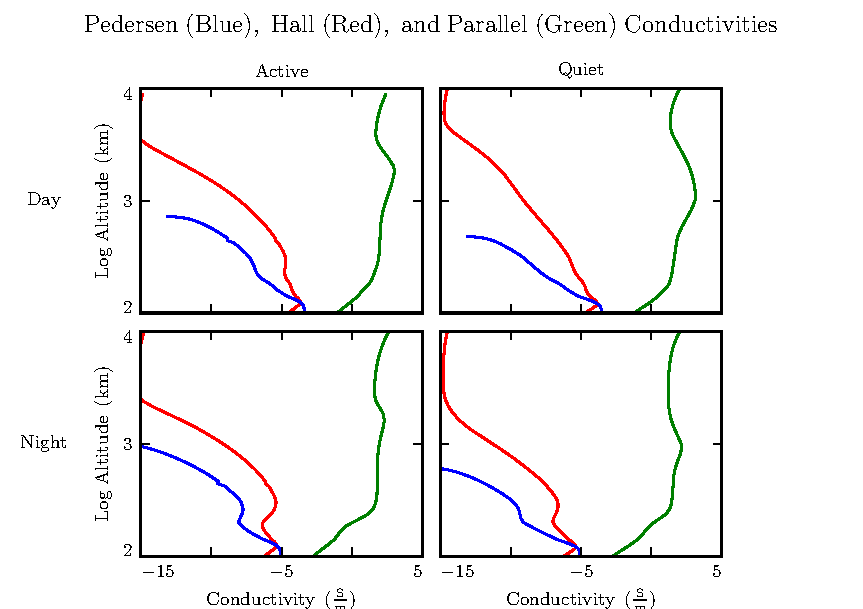
\includegraphics[width=\textwidth]{figures/sigma.pdf}
    \caption[Ionospheric Conductivity Profiles]{
      Ionospheric conductivity profiles, from \cite{lysak_2013}, or maybe \cite{kelley_1989}. 
    }
    \label{fig_sigma}
\end{figure}


% -----------------------------------------------------------------------------
% -----------------------------------------------------------------------------
% -----------------------------------------------------------------------------
\subsection{\Alfven Speed}

Number density is the sum of a plasmaspheric profile and a ``auroral'' profile. 

The mean molecular mass is based on eyeballing from \cite{lysak_2004}. He gives characteristic values at a few different altitudes. This has no visible effect on the code. 

This section isn't about the electric constant, even though that's what we read in. If it were, we would have to talk about the Boris correction. That's a few sections later. 

The low-density electric constant is read in from Bob/Kelley. It's then adjusted in accordance with the zeroth-order magnetic field strength and the local number density. The \Alfven speed is computed from $\va^2 \equiv \frac{1}{\mu_0 \ep}$. 

The Ionospheric \Alfven Resonator (IAR) is definitely included in this model, but it's not super important in practice. IAR modes resonate at $\sim\SI{1}{\Hz}$ and our driving is two orders of magnitude slower. 

NOTE: DO WE HAVE TO WORRY ABOUT PLASMA OSCILLATION IN THE IAR? 

% =============================================================================
% =============================================================================
% =============================================================================
\section{Maxwell's Equations}
  \label{sec_eqns}

The model simulates the evolution of electric and magnetic fields in accordance with Maxwell's equations. Specifically, magnetic fields are advanced using \farlaw, and electric fields with \amplaw. Kirchhoff's formulation of \ohmlaw ($\vec{J} = \tensor{\sigma} \cdot \vec{E}$) is used to eliminate the explicit current dependence in \amplaw. 
\begin{align}
  \ddt \vec{B} &= - \curl{E} &
  \tensor{\epsilon} \cdot \ddt \vec{E} &= \frac{1}{\mu_0} \curl{B} - \tensor{\sigma} \cdot \vec{E}
\end{align}

TALK ABOUT PRECOMPUTING COEFFICIENTS. 

TALK ABOUT HALF TIME STEP OFFSET?

Working only in terms of the covariant basis decreases our model's memory demands -- only one version of each field must be stored -- while simultaneously improving performance. 

% -----------------------------------------------------------------------------
% -----------------------------------------------------------------------------
% -----------------------------------------------------------------------------
\subsection{Magnetic Field}

Note that the \assign operator in \cref{def_assign} is used to indicate assignment, not equality. The values on the left hand side are new, and those on the right are old. New and old magnetic field values are offset by \dt. Electric field values are spaced halfway between them; compared to a magnetic field value, the electric field is either ahead or behind by $\frac{\dt}{2}$. 

In essence, this allows (with the reasonable assumption that the right hand side is varying slowly compared to \dt)
\begin{align}
  \ddt \vec{B} &= - \curl{E} \\
  \displaystyle\int_0^{\dt} dt \, \ddt \vec{B} &= - \displaystyle\int_0^{\dt} dt \, \curl{E} \\ 
  \left. \vec{B} \right|_{\dt} - \left. \vec{B} \right|_0 &= \left. - \dt \, \curl{E} \right|_{ \frac{\dt}{2} } \\
\intertext{Which we now write with the help of the \assign operator as}
  \label{def_assign}
  \vec{B} &\assign \vec{B} - \dt \, \curl{E}
\end{align}

In generalized coordinates, this looks like
\begin{align}
  \ddt B^i &= -\frac{ \varepsilon^{ijk} }{\jac} \partial_j E_k \\
\intertext{Or, eliminating contravariant terms, }
  \label{farlaw_ijk}
  \ddt B_i &= -\frac{ g_{ij} \varepsilon^{jkl} }{\jac} \partial_k E_l
\end{align}

Where summation is implied over repeated indeces, per Einstein's convention, and $\varepsilon^{ijk}$ is the Levi-Civita symbol \cite{einstein_1916}. 

Written out explicitly, and excluding metric tensor elements which are uniformly zero, \cref{farlaw_ijk} takes the form
\begin{align}
  \ddt B_1 &= - \frac{ g_{11} }{\jac} \lr{ \partial_2 E_3 - \partial_3 E_2 } - \frac{ g_{13} }{\jac} \lr{ \partial_1 E_2 - \partial_2 E_1 } \\
  \ddt B_2 &= - \frac{ g_{22} }{\jac} \lr{ \partial_3 E_1 - \partial_1 E_3 } \\
  \ddt B_3 &= - \frac{ g_{31} }{\jac} \lr{ \partial_2 E_3 - \partial_3 E_2 } - \frac{ g_{33} }{\jac} \lr{ \partial_1 E_2 - \partial_2 E_1 }
\end{align}

OR MAYBE
\begin{align}
  B_1 &\assign B_1 - \frac{g_{11} \dt}{\jac} \lr{ \partial_2 E_3 - \partial_3 E_2 } - \frac{g_{13} \dt}{\jac} \lr{ \partial_1 E_2 - \partial_2 E_1 } \\
  B_2 &\assign B_2 - \frac{g_{22} \dt}{\jac} \lr{ \partial_3 E_1 - \partial_1 E_3 } \\
  B_3 &\assign B_3 - \frac{g_{31} \dt}{\jac} \lr{ \partial_2 E_3 - \partial_3 E_2 } - \frac{g_{33} \dt}{\jac} \lr{ \partial_1 E_2 - \partial_2 E_1 }
\end{align}


% -----------------------------------------------------------------------------
% -----------------------------------------------------------------------------
% -----------------------------------------------------------------------------
\subsection{Parallel Electric Field}

The conductivity tensor couples the two perpendicular electric field components to one another, but doesn't couple them to the parallel electric field. As a result, the parallel component of \amplaw can be considered on its own. 
\begin{align}
  \label{amp_para}
  \ez \ddt E_\parallel &= \frac{1}{\mz} \lr{ \curl{B} }_\parallel - \sz E_\parallel
\end{align}

Assuming that $\lr{ \curl{B} }_\parallel$ varies slowly compared to \dt -- which it does, by construction -- \cref{amp_para} can be solved using integrating factors. 
\begin{align}
  E_\parallel &\assign E_\parallel \exp \arg{ \tfrac{- \sz \dt}{\ez} } + c^2 \dt \lr{ \curl{B} }_\parallel \exp \arg{ \tfrac{- \sz \dt}{2 \ez} }
\end{align}

Where of course $c^2 \equiv \frac{1}{\mz \ez}$. 

Note that $\lr{ \curl{B} }_\parallel$ is proportional to $\lr{ \curl{B} }_3$, and thus depends on both $\lr{ \curl{B} }^1$ and $\lr{ \curl{B} }^3$. Then in covariant terms
\begin{align}
  E_3 &\assign E_3 \exp \arg{ \tfrac{- \sz \dt}{\ez} } + c^2 \dt \lr{ g_{31} \frac{\partial_2 B_3 - \partial_3 B_2}{\jac} +  g_{33} \frac{\partial_1 B_2 - \partial_2 B_1}{\jac} } \exp \arg{ \tfrac{- \sz \dt}{2 \ez} }
\end{align}




For the aforementioned ionospheric profiles and time steps, $\frac{\sz \dt}{\ez}$ is never smaller than $10^3$. As a result, $\exp \arg{ \frac{- \sz \dt}{\ez} }$ is far too small to be stored in a double precision variable. That is, this simulation takes $E_\parallel$ to be uniformly zero. 

THIS MEANS THAT WE CAN'T TALK AT ALL ABOUT FIELD-ALIGNED CURRENTS. 

NOTE THAT WE WILL GET INTO THIS MORE IN \cref{ch_inertia}. 

Not unrelatedly, $\frac{\sz}{\ez}$ can also be written as $\frac{\op^2}{\nu}$; recall from \cref{def_basics} that the plasma frequency \op is given by $\op^2 \equiv \frac{n e^2}{\me \ez}$, and that the parallel conductivity $\sz$ is given by $\sz \equiv \frac{n e^2}{\me \nu}$ for collision frequency $\nu$. 

The plasma frequency is REALLY FAST. Near the ionospheric boundary the collision frequency is also pretty fast compared to the waves we're looking at, but not enough to overcome $\op^2$. 





% -----------------------------------------------------------------------------
% -----------------------------------------------------------------------------
% -----------------------------------------------------------------------------
\subsection{Perpendicular Electric Field}

The perpendicular electric field components are coupled by the conductivity tensor. 

... \\


\begin{align}
  \label{amp_perp}
  \ep \ddt \vec{E}_\bot &= \frac{1}{\mu_0} \lr{ \curl{B} }_\bot - \tensor{\sigma}_\bot \cdot \vec{E}_\bot
\end{align}

Cast in terms of the linear polarizations $E_x$ and $E_y$, this is a pair of coupled differential equations. However, in a circularly-polarized basis, the conductivity tensor is diagonal. Taking $E_\pm \equiv \frac{1}{ \sqrt{2} } \lr{E_x \pm i E_y}$, and defining components of \curl{B} analogously, \cref{amp_perp} can be written
\begin{align}
  \ep \ddt E_\pm &= \frac{1}{\mu_0} \lr{ \curl{B} }_\pm - \lr{ \sp \pm i \sh } E_\pm
\end{align}

Using integrating factors, and recalling $\va^2 \equiv \frac{1}{\mu_0 \ep}$, the new values of $E_\pm$ can be separated from the old. 
\begin{align}
  E_\pm &\assign E_\pm \exp \arg{- \tfrac{\sp \pm i \sh}{\ep} \dt} + \va^2 \dt \lr{ \curl{B} }_\pm \exp \arg{ - \tfrac{\sp \pm i \sh}{\ep} \tfrac{\dt}{2} }
\end{align}

As in \cref{def_assign}, \assign indicates that the left hand side is new, and the right hand side is old, with electric and magnetic fields offset from one another by $\frac{\dt}{2}$. 

Rotating from circular polarization to linear causes the imaginary terms within each exponential to cancel out, leaving sines and cosines. The expression can then be written
\begin{align}
  \label{eperp_tensor}
  \vec{E}_\bot &\assign 
  \tensor{R} \arg{ \tfrac{- \sh \dt}{\ep} } \cdot
  \vec{E}_\bot \exp \arg{ \tfrac{- \sp \dt}{\ep} } +
  \va^2 \dt \tensor{R} \arg{ \tfrac{- \sh \dt}{2 \ep} } \cdot
  \lr{ \curl{B} }_\bot \exp \arg{ \tfrac{- \sp \dt}{2 \ep} }
\end{align}

Where $\tensor{R}$ is the rotation matrix
\begin{align}
  \tensor{R} \arg{\theta} \equiv \mm{\cos\theta}{-\sin\theta}{\sin\theta}{\cos\theta}
\end{align}

This expression can then be mapped from the physical basis to the covariant basis, per \cref{def_h123}, to enable the evaluation of derivatives. Note that $E_x$ is parallel to $E^1$, which must then be expressed in terms of $E_1$ and $E_3$. This adds several terms to the expression. 
\begin{align}
  \begin{split}
    \label{e1_final}
    E_1 + \frac{ g^{13} }{ g^{11} } E_3 &\assign 
      \lr{ E_1 + \frac{ g^{13} }{ g^{11} } E_3 } \cos \arg{ \tfrac{- \sh \dt}{\ep} } \exp \arg{ \tfrac{- \sp \dt}{\ep} } \\
    & + \sqrt{ \frac{ g^{22} }{ g^{11} } } E_2 \sin \arg{ \tfrac{- \sh \dt}{\ep} } \exp \arg{ \tfrac{- \sp \dt}{\ep} } \\
    & + \frac{1}{ g^{11} } \frac{ \partial_2 B_3 - \partial_3 B_2 }{\jac} \cos \arg{ \tfrac{- \sh \dt}{2 \ep} } \exp \arg{ \tfrac{- \sp \dt}{2 \ep} } \\
    & + \sqrt{ \frac{1}{ g^{11} g^{22} } } \frac{ \partial_3 B_1 - \partial_1 B_3 }{\jac} \sin \arg{ \tfrac{- \sh \dt}{2 \ep} } \exp \arg{ \tfrac{- \sp \dt}{2 \ep} }
  \end{split} \\
  \begin{split}
    \label{e2_final}
    E_2 &\assign 
      - \sqrt{ \frac{ g^{11} }{ g^{22} } } \lr{ E_1 + \frac{ g^{13} }{ g^{11} } E_3 } \sin \arg{ \tfrac{- \sh \dt}{\ep} } \exp \arg{ \tfrac{- \sp \dt}{\ep} } \\
    & + E_2 \cos \arg{ \tfrac{- \sh \dt}{\ep} } \exp \arg{ \tfrac{- \sp \dt}{\ep} } \\
    & - \sqrt{ \frac{1}{ g^{11} g^{22} } } \frac{ \partial_2 B_3 - \partial_3 B_2 }{\jac} \sin \arg{ \tfrac{- \sh \dt}{2 \ep} } \exp \arg{ \tfrac{- \sp \dt}{2 \ep} } \\
    & + \frac{ \partial_3 B_1 - \partial_1 B_3 }{\jac} \cos \arg{ \tfrac{- \sh \dt}{2 \ep} } \exp \arg{ \tfrac{- \sp \dt}{2 \ep} }
  \end{split}
\end{align}

The $E_3$ dependence on the right hand side of \cref{e1_final} is resolved using the known value of $E_3$. Note that $E_3$ is parallel to $E_\parallel$, so decoupling them algebraically is trivial. 

% =============================================================================
% =============================================================================
% =============================================================================
\section{Driving}
  \label{sec_driving}

We have to get the energy in there somehow. Driving current is purely perpendicular. There is no component within the meridional plane (along the zeroth-order field or perpendicular to it). However, some effect is felt immediately on $E_x$ due to the Hall conductivity. 

% -----------------------------------------------------------------------------
% -----------------------------------------------------------------------------
% -----------------------------------------------------------------------------
\subsection{Outer Boundary Compression}

In the past, similar work has been done using compressional driving. 

This constrains the values of \azm that can be looked at. At large \azm, \Alfven waves can't propagate across field lines. They become purely guided. 

We can do some runs to show that this is the case. Can we also get it to fall out of the dispersion relation? The one from the previous chapter, not the generic \Alfven wave one. 

It's appropriate to drive with current because Pc4 pulsations are known to interact with energetic particles from the ring current and radiation belts. 

Substorm injections can cause azimuthal asymmetry in the ring current. 

% -----------------------------------------------------------------------------
% -----------------------------------------------------------------------------
% -----------------------------------------------------------------------------
\subsection{Ring Current Modulation}

We look at Sym-H to get an idea of the appropriate scale for current driving. We look at a few storms. 1 June 2013. 17 March 2015. 22 June 2015. 17 March 2013. A few in October and November 2012. 

We plot the power spectrum and basically do a fit for the top of the range of $\frac{1}{f}$ noise. This gives us a typical magnitude for oscillations on the order of a minute. 

This doesn't give us a characteristic spatial extent for ring current modulations -- Sym-H is a global index -- but we can eyeball the size of current fluctuations. We know the approximate size of the ring current, so we can go from ground-based field signature to current density in space pretty easily. 

There are a lot of parameters to play with. Since this is a linear code, we don't have to worry about ``sweet spots'' for nonlinear effects in the driving magnitude. And it doesn't look like the exact position or shape of the ring current has much qualitative effect on what we see. 

Looking at SYMH. Fourier series out to a period of about a minute. The power spectrum (judging from June 1-3 2013) gives you ~$10^{-2} (T/minutes)$. We can hand-wave a mapping from SYMH to the ring current. 
\begin{align}
  B & = \frac{\mu_0 I}{2 R}
\end{align}

With $B \sim \SI{2}{\nano\tesla}$, $R \sim \SI{4}{\RE}$, $A \sim \SI{1}{\RE\squared}$, we end up with $J \sim \SI{e-4}{\micro\ampere/\meter\squared}$. 

% =============================================================================
% =============================================================================
% =============================================================================
\section{Boundary Conditions}
  \label{sec_bcs}


The grid can't go on forever. There have to be special cases at the edges. 

% -----------------------------------------------------------------------------
% -----------------------------------------------------------------------------
% -----------------------------------------------------------------------------
\subsection{Parity and Interpolation}

At the inner and outer boundaries (that is, along the innermost and outermost field lines), as use Dirichlet and Neumann boundary conditions for electric and magnetic fields respectively. 

These are implemented in the differentiation and (parity) interpolation functions. 

Whenever we need to know the magnetic field just outside the grid boundary, we say that its value is the same as just inside the grid boundary, and its derivative is zero. Neumann. 

Conversely, we say that the electric field just outside the grid goes to 0, allowing us to compute the derivative from the value just inside the grid. Dirichlet. 

Dirichlet and Neumann could be flipped without much consequence. They're sorta arbitrary. But mixing up a term, so that they are no longer self-consistent, causes instability. 

Each field component is stored at only one parity in each direction. This is because of how curls line up. Adjacent values of $E_2$ just aren't really coupled to each other. 

This means that computing all of the parities isn't just unnecessary -- it's potentially unstable. The odd-by-odd grid and the odd-by-even grid are only weakly coupled, especially at large $r$, so they can drift apart. This can lead to problems in places where they do care about one another. This is documented... where??? 

This would be perfectly true if we were taking curls on an orthonormal grid, and if there was no Hall conductivity. As is, it's still pretty true. The contributions of off-parity terms tend to be small. 


% -----------------------------------------------------------------------------
% -----------------------------------------------------------------------------
% -----------------------------------------------------------------------------
\subsection{Coupling to the Atmosphere}

% note that, per lysak 2004, we are assuming no vertical current through the ionospheric current sheet. 

Per Maxwell's equations, $\div{B}=0$. We further assume that there are no currents flowing in the atmosphere, giving $\curl{B}=0$. These conditions together guarantee the existence of a scalar magnetic potential, $\Psi$, which satisfies Laplace's equation, $\nabla^2 \Psi = 0$ and $\vec{B} = \grad{\Psi}$. 

Separating out the $r$ and $\phi$ components of Laplace's equation, the $\theta$ component of the equation can be written as a differential equation in terms of $u \equiv \cos\theta$: 
\begin{align}
  \frac{d}{d u} \lr{ \lr{1 - u^2} \frac{d}{d u} Y_\nu } - \frac{m^2}{1 - u^2} Y_\nu & = - \nu \lr{\nu + 1} Y_\nu
\end{align}

This can be solved numerically on our discrete grid, providing us with eigenvectors and eigenvalues ($Y_\nu$ and $\nu$ respectively). We can then write $\Psi$ in terms of those harmonics: 
\begin{align}
  \Psi \lr{r, \theta} = & \displaystyle\sum_\nu \lr{ \alpha_\nu r^\nu + \beta_\nu r^{-\nu-1} } Y_\nu \lr{\theta}
\end{align}

We will rearrange this expression in order to compute $\Psi$ each time step as a linear combination of the radial magnetic field values at $R_I$. 

We defined $\vec{B} = \grad{\Psi}$, so $B_r = \dd{r} \Psi$. 

The ground is perfectly conducting, so $B_r \lr{R_E} = 0$. 

...

We don't need to show algebra, but we should show the final expression. 

...

Jump condition over the ionospheric current sheet. This comes from integrating \amplaw... ?

